\chapter{Validation (part 1): model selection and model
assessment}\label{ch-09}

Validation was introduced in
\href{04\%20-\%20Generalizzazione\%20e\%20validazione\%20(introduzione)}{04
- Generalisation and validation (introduction)}; these lectures go into
more depth, because it is indispensable for the project and for any
serious application of ML. The two goals (model selection and model
assessment) are restated, a counterexample shows how easy it is to
obtain wrong estimates, \textbf{grid search} and \textbf{K-fold
cross-validation} are introduced, and sampling, scarce data and error
measures are discussed.

\section{Preamble: bias and variance}\label{premessa-bias-e-varianza}

The \textbf{bias-variance} decomposition (which will have a dedicated
lecture) is a useful framework for understanding why estimating the
performance of a model is difficult: it shows the role of the different
\textbf{realisations of the training set} and, once again, the
trade-off between fitting capability (bias) and model flexibility
(variance).

\begin{figure}[htbp]
\centering
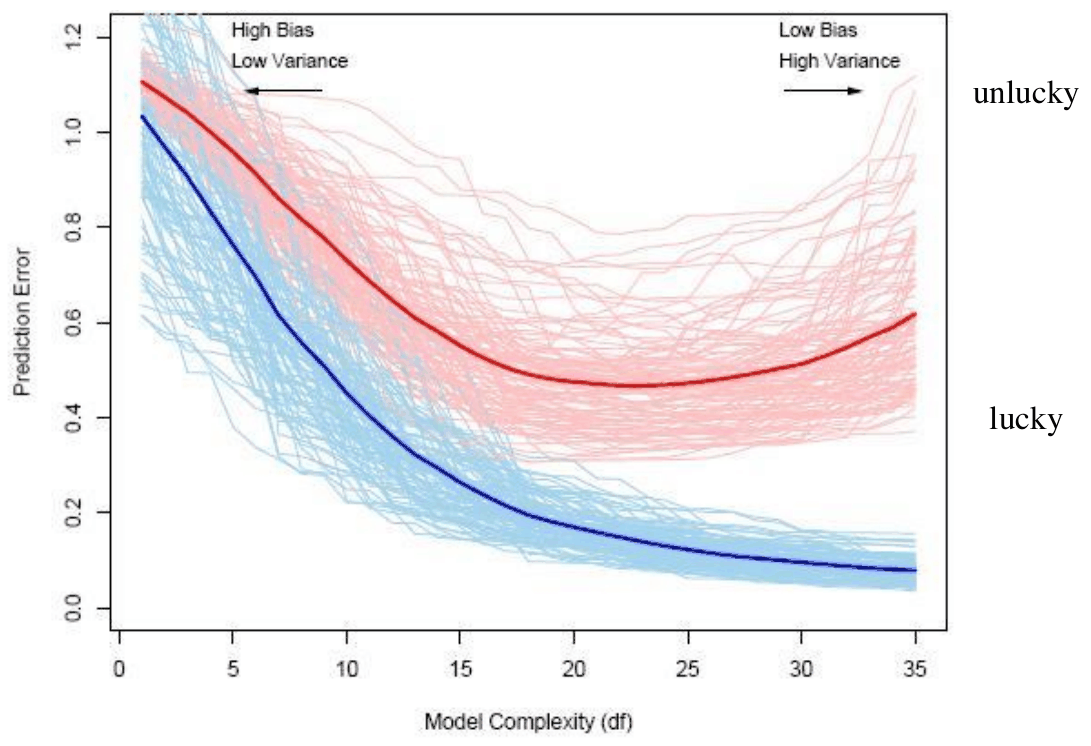
\includegraphics[width=0.71\linewidth,height=0.42\textheight,keepaspectratio]{images/09-val1_bias-varianza.png}
\caption{Training (light blue) and test (red) error on 100 different
training sets as complexity grows (Hastie et al., Fig.\ 7.1). With a
complex model the bias is low but the variance is high: depending on
the sample one can be ``lucky'' or ``unlucky''.}
\end{figure}

The figure shows an important fact: for the same complexity, the test
error varies a lot from one training set to another, especially for
complex models. A single measurement can be lucky or unlucky.

\section{Motivations}\label{motivazioni}

We look for the solution with the minimum prediction (test) error,
balancing \textbf{fit to the training data} and \textbf{model
complexity}. The training error \textbf{is not a good estimate} of the
test error: at first there is too much bias (underfitting, high
training error), then too much variance (low training error but
overfitting).

Assuming we have a hyperparameter \(\theta\) (implicit or explicit)
that controls the complexity of the model, we want the value of
\(\theta\) that minimises the test error. We therefore need methods to
\textbf{estimate the expected error} of a model (or of each model of a
class, or of a set of models).

\subsection{How to estimate}\label{come-stimare}

\begin{itemize}
\tightlist
\item
  \textbf{Analytically}: AIC and BIC criteria (\emph{Akaike/Bayesian
  Information Criterion}, limited to models linear in the parameters),
  MDL (\emph{Minimum Description Length}), \textbf{SRM}
  (\emph{Structural Risk Minimization}) with the VC-dimension (see the
  lecture on SLT).
\item
  \textbf{Empirically}, on the data, through \textbf{resampling}
  (direct estimation of the out-of-sample error):
  \textbf{cross-validation} (hold-out, K-fold, \ldots) and
  \textbf{bootstrap}.
\end{itemize}

\section{The two goals of
validation}\label{i-due-obiettivi-della-validazione}

\begin{boxwarning}{The most important slide of the course}

After training the models on the training set:

\begin{itemize}
\tightlist
\item
  \textbf{Model selection}: estimate the performance (generalisation
  error) of different models in order to \textbf{choose the best one}.
  It includes searching for the best \textbf{hyperparameters} (degree
  of the polynomial, number of units of a network, \(\lambda\),
  \(\eta\), \ldots). \emph{Returns a model.}
\item
  \textbf{Model assessment}: having chosen the final model (or a class
  of models), \textbf{estimate its prediction error} (risk) on new test
  data, as a measure of the quality of the chosen model. \emph{Returns
  an estimate.}
\end{itemize}

\textbf{Golden rule}: keep the goals separate and use \textbf{separate
data sets} in each phase.

\end{boxwarning}

\subsection{Hold-out}\label{hold-out}

If there are enough data, the dataset is split into three
\textbf{disjoint} sets, for example 50\% TR, 25\% VL, 25\% TS:

\begin{itemize}
\tightlist
\item
  \textbf{TR} (\emph{training set}): to fit the model, i.e.\ minimise
  the SLT \(R_{emp}\) {[}\textbf{training}{]};
\item
  \textbf{VL} (\emph{validation} or \emph{selection set}): to choose
  the best model among different models and hyperparameter
  configurations {[}\textbf{model selection}{]};
\item
  \textbf{TS} (\emph{test set}): to estimate the generalisation error
  of the final model, i.e.\ estimate the SLT \(R\) {[}\textbf{model
  assessment}{]}.
\end{itemize}

TR and VL together form the \textbf{development/design set}, used to
build the final model.

\begin{boxnote}{Two clarifications}

\begin{enumerate}
\def\labelenumi{\arabic{enumi}.}
\tightlist
\item
  The estimate made on VL serves \textbf{only} for model selection: it
  is not a good estimate for assessment.
\item
  The results on TS \textbf{cannot} be used for model selection. If
  this is done, it is no longer a test set: let us call it a validation
  set.
\end{enumerate}

\end{boxnote}

\subsection{Test or model selection?}\label{test-o-model-selection}

What happens if the test set is used in a repeated design cycle (try,
look at the test, change, try again)? One is doing \textbf{model
selection}, not a reliable evaluation, and we could not do this on
future examples. The error on the test set used in this way is a
\textbf{too optimistic estimate} of the true error. It is like an exam
exercise whose solutions have been seen: it is no longer a test! Hence
the concept of \textbf{blind test set}, used in ML competitions.

\begin{figure}[htbp]
\centering
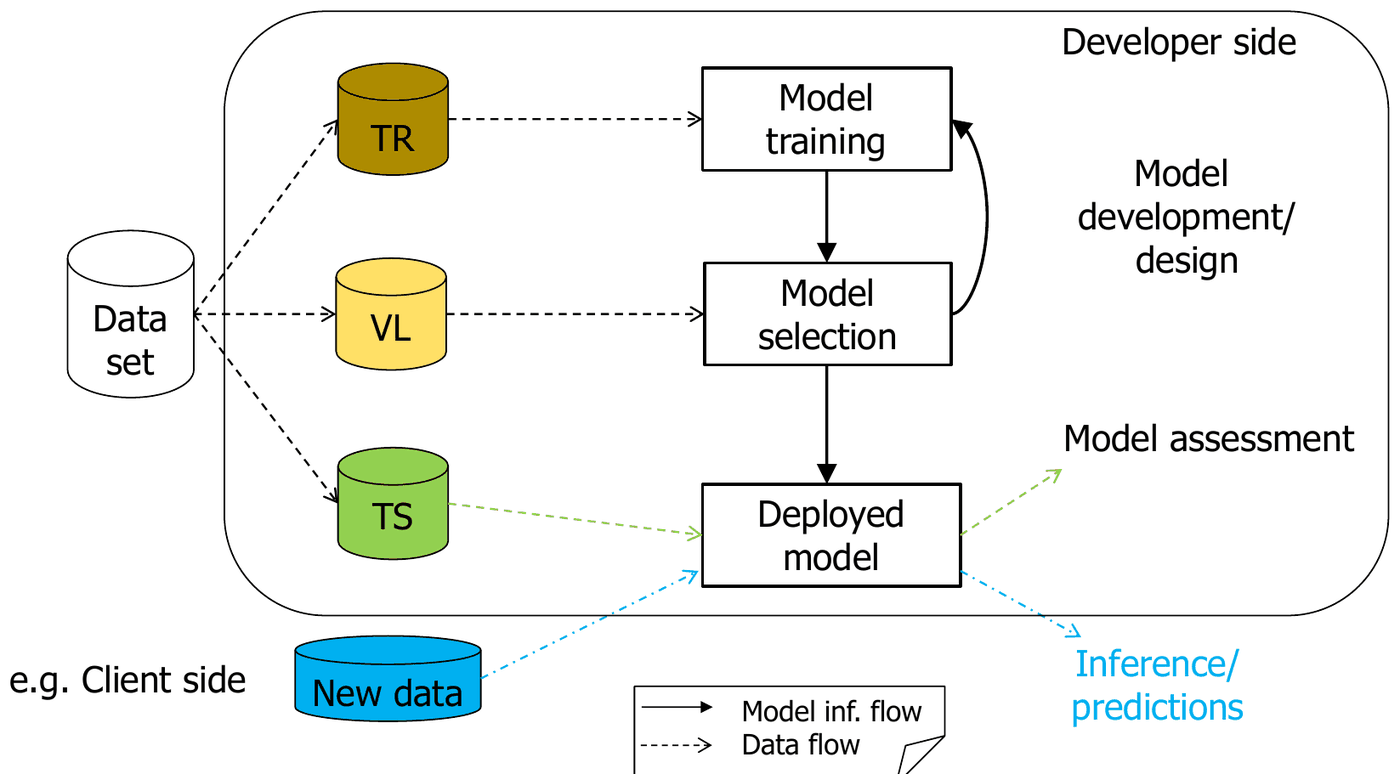
\includegraphics[width=0.80\linewidth,height=0.42\textheight,keepaspectratio]{images/04-l4_schema-tr-vl-ts.png}
\caption{Role of TR, VL and TS (taken from lecture 4).}
\end{figure}

\section{An instructive counterexample}\label{un-controesempio-istruttivo}

\begin{boxexample}{The random target counterexample}

\begin{itemize}
\tightlist
\item
  20--30 examples, \textbf{1000 input variables} with random values;
\item
  \textbf{random} 0/1 target.
\end{itemize}

A model is selected that uses \textbf{a single} input variable, the one
that by pure chance ``guesses'' the target at 99\% (or 100\%) on any
subsequent split into TR, VL and TS. Perfect result? What is wrong?

The 99--100\% is \textbf{not} a good estimate of the test error: the
true one is \textbf{50\%} (the target is random, no model can do
better than a coin). On a truly new external test set one would get
50\%.

\end{boxexample}

There are two errors:

\begin{enumerate}
\def\labelenumi{\arabic{enumi}.}
\tightlist
\item
  the error estimate on TR and VL \textbf{is not} a good estimate of
  the risk;
\item
  using \textbf{the whole dataset} for feature or model selection
  \textbf{compromises the estimate} (biased estimate, called
  \emph{subset selection bias}): the test set was used
  \textbf{implicitly} at the beginning, in the choice of the variable.
  The test set must be separated \textbf{in advance}, before
  \textbf{any} model selection, including \textbf{feature selection}.
\end{enumerate}

With 1000 random variables and only 20 patterns, it is almost certain
that one variable will coincide by chance with the target on most
patterns. Since the choice is made looking at \textbf{all} the data,
that variable ``works'' on any subsequent partition. On truly new
patterns (TS1, TS2, TS3 in the table of the slide) the same variable
has accuracies of 100\%, 33\%, 66\%: pure chance.

\begin{boxwarning}{Warning}

Here we are discussing the \textbf{correctness of the estimate}, not
the possibility of solving the task. K-fold CV and other techniques
\textbf{do not} solve the problem if the selection is made before the
split (on the contrary, they can confuse things even more).

\end{boxwarning}

\section{Grid search}\label{grid-search}

\textbf{Hyperparameters} are parameters not learned directly by the
algorithm; they are fixed by searching in the \textbf{hyperparameter
space}, naturally through model selection on a validation set.

\textbf{Exhaustive grid search} generates all candidates from a grid
of values. Trivial example with number of units and \(\lambda\):

{\def\LTcaptype{none} % do not increment counter
\begin{longtable}[]{@{}llll@{}}
\toprule\noalign{}
Units ~\(\lambda\) & 0.1 & 0.01 & 0.001 \\
\midrule\noalign{}
\endhead
\bottomrule\noalign{}
\endlastfoot
1 unit & Res1 & Res4 & Res7 \\
10 units & Res2 & Res5 & Res8 \\
100 units & \textbf{Res3} & Res6 & Res9 \\
\end{longtable}
}

If the best result (on validation) is Res3, the configuration (100
units, \(\lambda = 0.1\)) wins. It must be \textbf{automated}, and it
is easy to \textbf{parallelise} (the trials are independent).

The cost can be high: it is the Cartesian product of the values, i.e.\
\((\#\text{values})^{\#\text{hyperparameters}}\). With 3 values for 2
hyperparameters there are \(3^2 = 9\) trials; with 5--6
hyperparameters of 10 values each it becomes prohibitive. Therefore:

\begin{itemize}
\tightlist
\item
  some hyperparameters can be fixed in a preliminary experimental
  phase, if they prove to be of little relevance (with caution, see the
  sequential selection error in part 3);
\item
  \textbf{two (or more) levels of nested grid search} are used: first
  a \textbf{coarse} search over all combinations (for example with
  exponentially growing values) to find the good regions, then
  \textbf{finer} searches over smaller and smaller intervals, always
  considering \textbf{all} the significant hyperparameters together.
\end{itemize}

\subsection{Alternatives to grid
search}\label{alternative-alla-grid-search}

Grid search is very useful for \textbf{observing the behaviour} of the
model as the hyperparameters vary (fundamental for understanding), but
it is expensive and scales poorly with the number of hyperparameters.
Alternatives:

\begin{itemize}
\tightlist
\item
  \textbf{random search} (Bergstra and Bengio, 2012): it avoids
  resampling the same values of an influential hyperparameter when
  others are not influential, and it allows fixing the \textbf{budget}
  of trials independently of the number of hyperparameters;
\item
  \textbf{automatic} search: Bayesian and evolutionary approaches,
  configuration evaluation methods (e.g.\ Hyperband).
\end{itemize}

Libraries such as Keras Tuner and scikit-learn include many
alternatives (towards \textbf{AutoML}), but they should not be used
uncritically: grid search teaches more at first approach.

\begin{figure}[htbp]
\centering
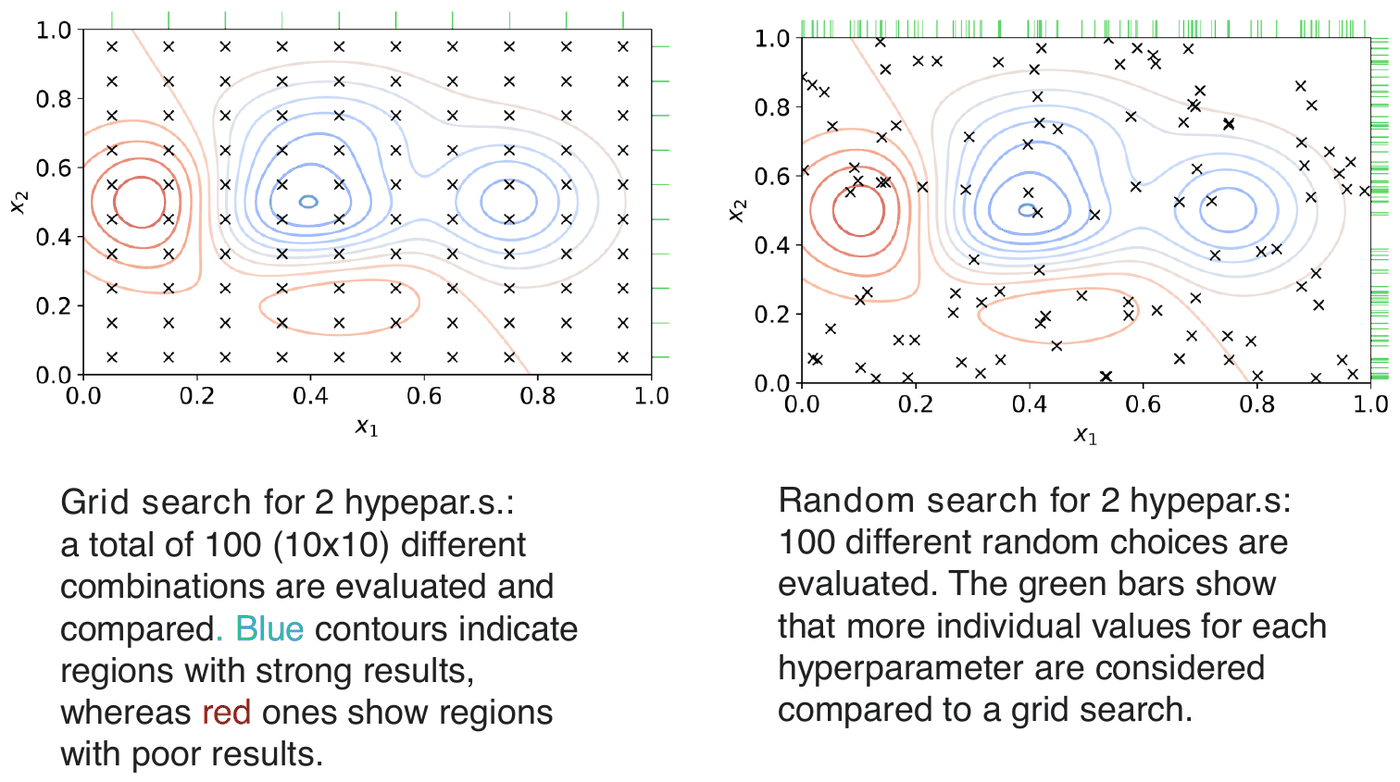
\includegraphics[width=0.91\linewidth,height=0.42\textheight,keepaspectratio]{images/09-val1_grid-random.png}
\caption{Grid search and random search with 100 trials each: random
search explores many more distinct values of each hyperparameter (green
bars).}
\end{figure}

\begin{boxtip}{Why random search works}

If only one of the two hyperparameters really matters, the 10×10 grid
tries only \textbf{10 distinct values} of it (the other 90 trials
repeat the same values while varying the useless hyperparameter),
whereas random search tries \textbf{100}.

\end{boxtip}

\section{K-fold cross-validation}\label{k-fold-cross-validation}

\subsection{How much data is needed?}\label{quanti-dati-servono}

Hold-out requires enough data for three meaningful partitions. How
many? It depends on the complexity of the model and on the
signal-to-noise ratio (few are needed for a linear model on a
noise-free linearly separable task). What to do if there are not
enough data? And how to avoid depending on the \textbf{particular
partition} chosen? K-fold CV helps.

\begin{boxnote}{Terminology}

``Cross-validation'' denotes both an \textbf{approach} to model
selection based on direct estimation of the error through resampling
(rather than analytical), and more specifically the
\textbf{implementations} that establish how to split the data for
selection and for evaluation (for example K-fold CV).

\end{boxnote}

\subsection{Recap}\label{richiamo}

\(D\) is split into \(K\) mutually exclusive subsets
\(D_1,\dots,D_K\); for each \(i\) one trains on \(D \setminus D_i\) and
evaluates on \(D_i\). In this way all data are used both for training
and for evaluation. One does not obtain a \textbf{single model} (there
is one per fold), but one also obtains a \textbf{variance} (standard
deviation) over the folds for one's class of models: the result is
reported as \textbf{mean ± standard deviation}. It can be used both for
the validation set and for the test set.

Issues: how many folds (3, 5, 10, \ldots, \emph{leave-one-out})? The
computational cost is often high. It can be combined with a validation
set or a double K-fold CV can be performed.

\subsection{A complete example of selection and
assessment}\label{un-esempio-completo-di-selezione-e-valutazione}

\begin{enumerate}
\def\labelenumi{\arabic{enumi}.}
\tightlist
\item
  Split the data into \textbf{TR} and \textbf{TS} (here with hold-out,
  but it could be a K-fold).
\item
  \textbf{Model selection}: use a K-fold CV \textbf{internal} to TR
  (which in each fold produces new TR and VL) to find the best
  hyperparameters with a \textbf{grid search}. For each cell of the
  grid (e.g.\ \(\lambda = 0.1\), 20 units) an entire K-fold CV is run;
  the configuration with the \textbf{best mean validation error} over
  the folds is chosen.
\item
  Retrain the final model on the \textbf{whole} original \textbf{TR}.
\item
  \textbf{Model assessment}: evaluate it on the \textbf{external TS}.
\end{enumerate}

(Can one then retrain again on all the data? We will see this in the
next part.)

\section{Special cases}\label{casi-particolari}

\subsection{Lucky or unlucky
sampling}\label{campionamento-fortunato-o-sfortunato}

To avoid depending on the particular partition:

\begin{itemize}
\tightlist
\item
  \textbf{Stratification}: grouping the population into homogeneous
  subgroups before sampling. For classification: in each partition (TR
  and TS in hold-out or CV) each class is represented roughly in the
  same proportions as in the full dataset.
\item
  Check the composition of the folds: the \textbf{order of the data}
  could have a meaning (e.g.\ data sorted by class or by time).
\item
  \textbf{Repeated hold-out or CV}: repeat the split with different
  random samplings (e.g.\ repeat the CV 10 times) and average the
  results. Useful above all for \textbf{comparing different models}.
\end{itemize}

\subsection{Very few data}\label{pochissimi-dati}

With very few data it is hard to say whether a sample is
representative. Besides stratification, avoid (or take into account in
the evaluation): classes or features missing in the training data;
special classes not sampled in TR or TS; known outliers that affect the
mean of the test results; conversely, selecting only ``easy'' cases.

Even a \textbf{blind test set} can be misleading if it comes from a
different distribution, is measured with different scales or
tolerances, is not cleaned or pre-processed, or requires
\textbf{extrapolation} (out-of-range data).

\section{Error measures for
evaluation}\label{misure-derrore-per-la-valutazione}

\textbf{Classification} (see the first lectures): accuracy (or error
rate, often in \%), confusion matrix, specificity, sensitivity, ROC
curve.

\textbf{Regression}, with residual \(r_i = y_i - o_i\) (\(y\) target,
\(o\) output):

\begin{itemize}
\tightlist
\item
  \textbf{MSE} \(= \text{mean}_i[r_i^2]\) and its square root
  \textbf{RMS} (or \(S\));
\item
  \textbf{mean absolute error} (MAE) \(= \text{mean}_i[|r_i|]\);
\item
  \textbf{maximum absolute error} \(= \max_i |r_i|\);
\item
  \textbf{correlation coefficient} \(R\) (and \textbf{coefficient of
  determination} \(R^2\)), for example \(R = \sqrt{1 - S^2/S_y^2}\),
  with \(S_y^2 = \text{mean}_i[(y_i - \bar y)^2]\) the variance of the
  target: it measures the degree of linear dependence between \(y\) and
  \(o\), in \([0,1]\), where 1 is best;
\item
  \textbf{outputs versus targets} plots;
\item
  statistical tests and significance analysis.
\end{itemize}

\begin{boxnote}{Bootstrap}

Another approach is the \textbf{bootstrap}: random resampling
\textbf{with replacement}, repeated to obtain different (validation or
test) subsets.

\end{boxnote}

\begin{boxabstract}{The two golden rules}

\begin{itemize}
\tightlist
\item
  The result on \textbf{TR} is not a good estimate of that on VL and
  TS.
\item
  The result on \textbf{VL} is not a good estimate of that on TS.
\end{itemize}

Therefore: \textbf{do not use validation set results for estimating the
risk} (model assessment), and \textbf{do not use test set results for
model selection}, in any form. In a single rule: \emph{keep the goals
separate and use separate sets in each phase.}

\end{boxabstract}

\begin{boxquestion}{Possible exam questions}

\begin{itemize}
\tightlist
\item
  Difference between model selection and model assessment; why are
  separate sets needed?
\item
  Describe the random target counterexample: what are the two errors?
\item
  What is grid search? How can its cost be reduced? Advantages of
  random search.
\item
  Describe K-fold CV and a complete example of selection and
  assessment.
\item
  What is stratification?
\item
  Which error measures are used for regression?
\end{itemize}

\end{boxquestion}
